
	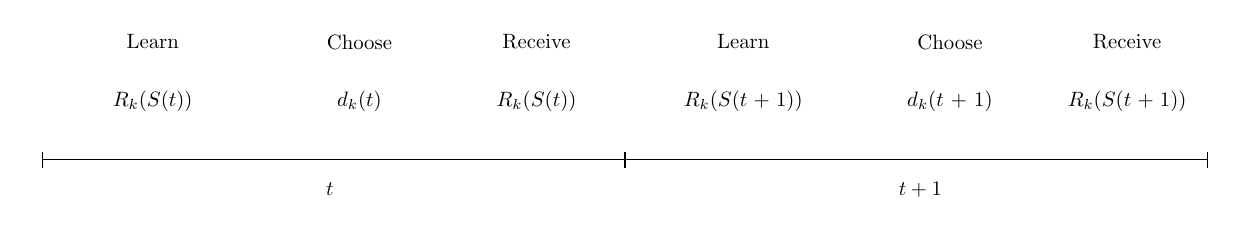
\begin{tikzpicture}[scale=1.0, every node/.style={scale=0.75}]

	\tikzset{
	eqblock/.style={text width=3cm,align=center}
	}

	% Nodes
	\node (left) {};
	\node[node distance=10cm, right of=left] (mid) {};
	\node[node distance=10cm, right of=mid] (right) {};

	\node[node distance=5cm, right of=left, yshift=-.5cm] (t1) {$t$};
	\node[node distance=5cm, right of=mid, yshift=-.5cm] (t2) {$t+1$};

	\node[eqblock, above of=left, xshift=2.0cm] (eq1) {$R_k(S(t))$};
	\node[eqblock, above of=left, xshift=5.5cm] (eq2) {$d_k(t)$};
	\node[eqblock, above of=left, xshift=8.5cm] (eq3) {$R_k(S(t))$};
	\node[eqblock, above of=mid, xshift=2.0cm] (eq4) {$R_k(S(t+1))$};
	\node[eqblock, above of=mid, xshift=5.5cm] (eq6) {$d_k(t+1)$};
	\node[eqblock, above of=mid, xshift=8.5cm] (eq5) {$R_k(S(t+1))$};

	\node[above of=eq1, node distance=1cm] (text2) {Learn};
	\node[above of=eq2, node distance=1cm] (text3) {Choose};
	\node[above of=eq3, node distance=1cm] (text1) {Receive};
	\node[above of=eq4, node distance=1cm] (text4) {Learn};
	\node[above of=eq6, node distance=1cm] (text5) {Choose};
	\node[above of=eq5, node distance=1cm] (text6) {Receive};

	% Lines
	\draw[|-|] (left) -- (mid.center);
	\draw[|-|] (mid.center) -- (right);

	\end{tikzpicture}
